\section{Encoding Variable-length Identifiers}\label{sec:identifiers}
\subsection{Allowing flexibility in identifiers' lengths}
In this section, we describe an enhanced encoding technique that enables further reduction in the required tag width.  While maintaining the ability to distinguish between different supersets, we allow their distinct identifiers to be of a variable length. We describe a simple condition on the identifiers that enable such a distinction. 

Consider the supersets from Table~\ref{Table_variable_a}, each described as a set of attributes. The largest of the $N=4$ supersets has five attributes. 
If fixed-length identifiers of $\left \lceil \log_2(N) \right \rceil = 2$ bits 00, 01, 10 and 11 are allocated then we derive a maximal width of 2 + 5 = 7 bits, as illustrated in Table~\ref{Table_variable_b}. 
Note that the observed total width for several of the subsets is shorter than the maximal.
In the general case, with fixed-length identifiers, given $N$ supersets of size $\ell_1, \ldots, \ell_N$ the required width is determined by the largest superset and equals 
 $W_{f} = \left \lceil \log_2(N) \right \rceil + \max_{i \in [1,N]} \ell_i$. 

In Table~\ref{Table_variable_c} variable-length identifiers 0, 10, 110 and 110 are used. This enables to reduce the maximal width to only 6 bits by allocating the largest supersets shorter identifiers. 
Notice that the identifiers are selected such that none of them is a prefix (start) of the other, i.e., the identifiers are codewords in a prefix code.
Such a selection of the identifiers enables to distinguish between the supersets for any value of their bit masks as the second part of the tag. 



%\begin{table}[t!]
%
%
%\centering
%subfigure[Supersets]{
%\begin{tabular}{|c|}
%\hline
%Superset elements\\
%\hline
%A B C\\
%C D\\
%E F\\
%W X Y Z\\
%\hline
%\end{tabular}
%}\\
%\end{table}








\begin{table}[t!]
\small

\centering
\begin{subtable}[t]{0.35\linewidth}
\caption{Supersets}\label{Table_variable_a}
\begin{tabular}{|c|}
\hline
Superset elements\\
\hline
A B C\\
C D\\
E F\\
W X Y Z\\
\hline
\end{tabular}
\end{subtable}\\


\begin{subtable}[t]{0.49\linewidth}
\caption{Fixed-length Identifiers}\label{Table_variable_b}
\begin{tabular}{|c|c|}
\hline
Identifier   &  Superset\\
\hline
00 & A B C\\
01 &  C D\\
10 &  E F\\
11 &  W X Y Z\\
\hline
\end{tabular}
\end{subtable}
\hfill
\begin{subtable}[t]{0.49\linewidth}
\caption{Variable-length Identifiers}\label{Table_variable_c}
\begin{tabular}{|c|c|}
\hline
Identifier   &  Superset\\
\hline
10 & A B C\\
110 &  C D\\
111 &  E F\\
0 &  W X Y Z\\
\hline
\end{tabular}
\end{subtable}

\caption{Illustration of variable-length identifiers for supersets. While with fixed-length identifiers the maximal width in (B) is 6 bits, with variable-length identifiers it is reduced in (C) to only 5 bits.
}\label{Table_variable}
\end{table}


yeah

\begin{figure}[t!] 
\begin{minipage}{1\linewidth}
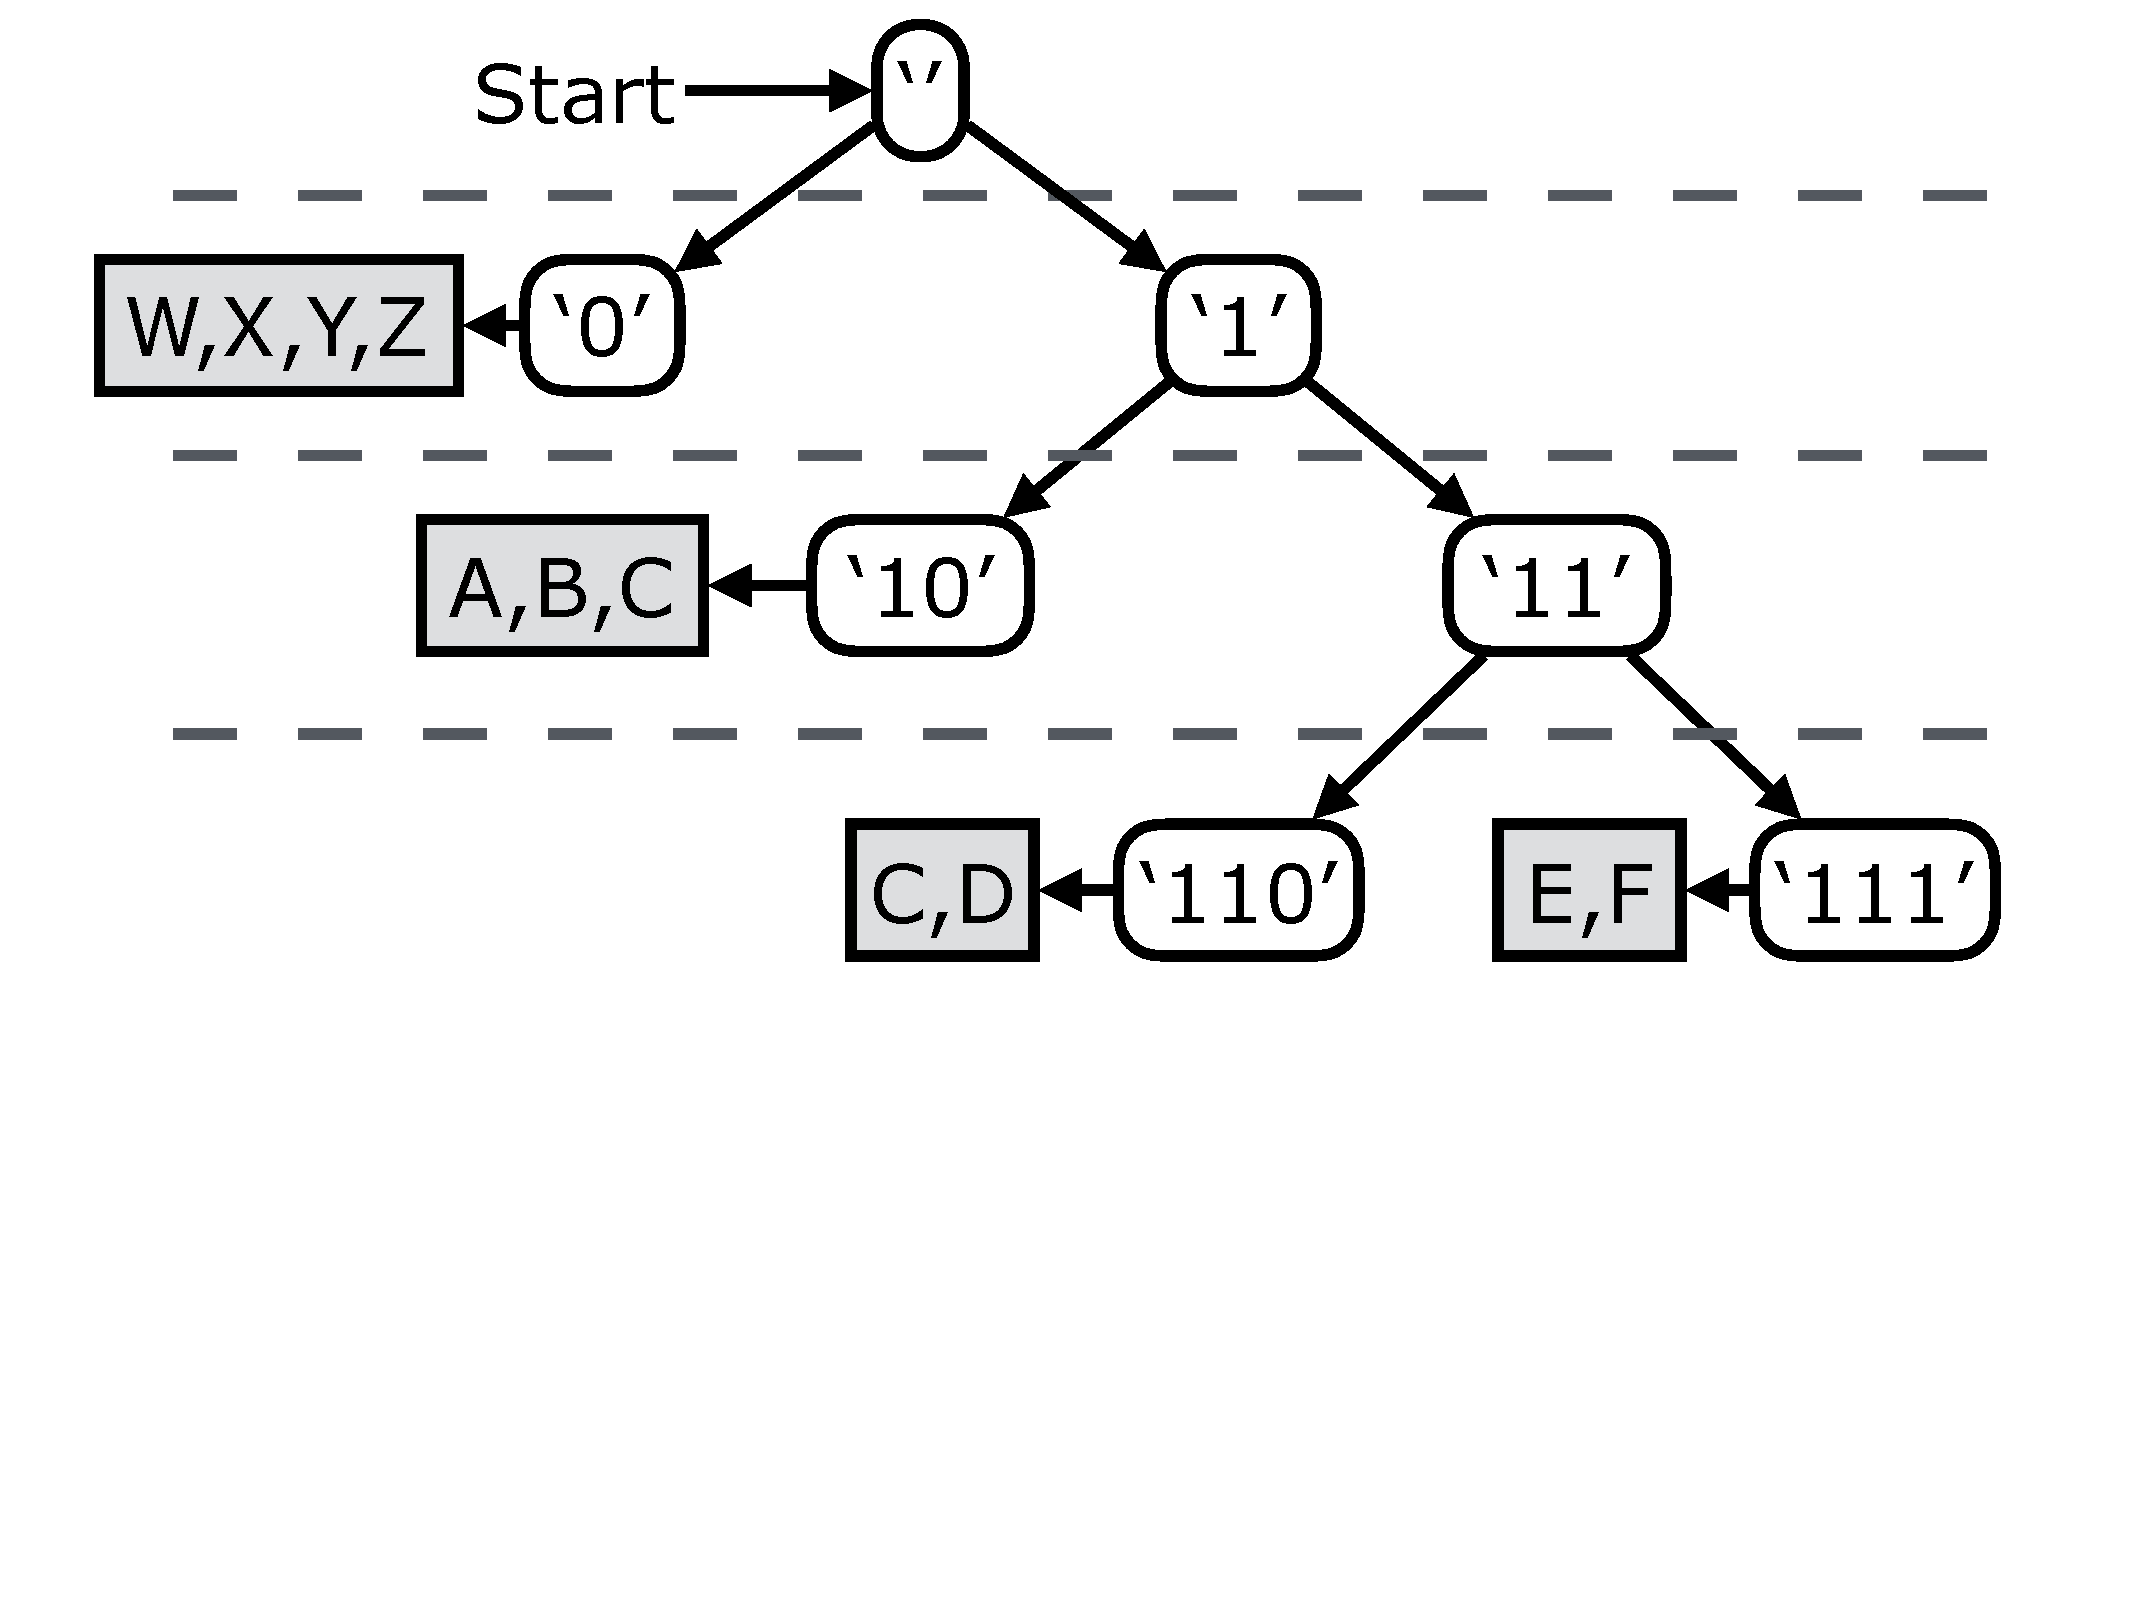
\includegraphics[trim={0 10cm 0 0}, clip, width=\linewidth]{figures/code_tree}
\end{minipage} 
\caption{An example prefix code tree, based upon the prefix code identifiers from Table~\ref{Table_variable_c} which are used to identify the attribute sets $[A,B,C]$, $[C,D]$, $[E,F]$ and $[W,X,Y,Z]$. This figure shows how reading a codeword corresponds to traversing a binary tree, starting at the root. By using such a code, larger sets are able to receive smaller identifiers, improving maximal  tag width.}
\label{fig:code_tree}
\end{figure}


Kraft's inequality~\cite{abramson} formally determines the existence of a prefix code with codewords of given lengths. It says that a code with $N$ codewords of lengths 
 $L_1, L_2, \ldots, L_N$ exists 
iff the following inequality holds:
$$ \sum_{i = 1}^{N}{2^{-L_i}} \le 1. $$

For instance, the lengths of the identifiers in Table~\ref{Table_variable_c} satisfy $2^{-1} + 2^{-2} + 2^{-3} + 2^{-3} = 1$.

This also enables us to exactly calculate the minimal width $W_{v}$ that can be achieved for a given $X$ supersets of size $\ell_1, \ldots, \ell_X$  using variable-length identifiers as described in the following property.

\begin{property}
For given supersets of size $\ell_1, \ldots, \ell_N$ the optimal (minimal) tag width that can be derived using variable-length identifiers is given by 
\begin{equation} \label{eq2}
W_{v}  = \left \lceil \log_2 \sum_{i = 1}^{N}{2^{\ell_i}} \right \rceil. \nonumber 
\end{equation}
\label{property_variable_length_minimal_tag}
\end{property} 
\bp
A width of $W_{v}$ allows assigning an identifier of length  $W_{v} - \ell_i$ to the $i$-th superset. By Kraft's inequality the width  $W_{v}$ must satisfy
\begin{equation} \label{eq1}
\begin{split}
1 &\ge \sum_{i = 1}^{N}{2^{-(W_{v}-\ell_i)}} = 2^{-W_{v}} \cdot \sum_{i = 1}^{N}{2^{\ell_i}}. \nonumber 
%  \Leftrightarrow 2^{W_{v}}  &\ge \sum_{i = 1}^{N}{2^{\ell_i}}  \nonumber \\
%  \Leftrightarrow W_{v}  &\ge \left \lceil \sum_{i = 1}^{N}{2^{\ell_i}}  \right \rceil \nonumber 
\end{split}
\end{equation}
Accordingly we have $2^{W_{v}}  \ge \sum_{i = 1}^{N}{2^{\ell_i}}$. Since $W_{v}$ is defined as the minimal possible width with that property the result follows.
\ep

%In the general case, with fixed-length identifiers, given $X$ supersets of size $\ell_1, \ldots, \ell_X$ the required width is determined by the largest superset and equals 
% $W_{f} = \left \lceil \log_2(X) \right \rceil + \max_{i \in [1,X]} \ell_i$. 
 
Since the fixed-length identifiers is a special case of the variable-length identifiers then necessarily $W_{v} \le W_{f}$. 

A selection of variable-length identifiers satisfying Kraft's inequality can be described as a subset of leaves in a binary tree. 
A path from the root node to a node corresponds to a binary string where visits of the left child or the right child of a node stand for bits of 0 and 1, respectively. 
The path length  to a leaf corresponds to the identifier length in bits.
Fig.~\ref{fig:code_tree} illustrates the corresponding tree for the four identifiers from Table~\ref{Table_variable_c}. 
Shorter identifiers appear more to the left in the tree.

For given supersets, after calculating $W_{v}$ as the minimal possible width enabled by variable-length identifiers we can easily find identifiers that realize it. We first calculate for a superset of size $\ell_i$ the (maximal) allowed length $W_{v} - \ell_i$. We sort the identifiers in an ascending length order. We consider a binary tree and while beginning from the root node, we relate to the next identifier the most left available leaf that its depth equals the length of the current identifier. We assign as the identifier the binary string obtained by the path from the root to the leaf.
 
\subsection{Optimizing Selection of Supersets}
In the selection of the supersets we would like to enable the existence of a short as possible tag. By Property~\ref{property_variable_length_minimal_tag} the number of supersets and their identities should be selected such that their sizes $\ell_1, \ldots, \ell_N$ minimize the term $T = \sum_{i = 1}^{N}{2^{\ell_i}}$. 

We describe a simple scheme to determine the supersets for a given (distinct) input sets $s_1, \ldots, s_N$. We first examine whether $s_i \subset s_j$ for some two sets. In this case, we can use $s_j$ as the superset for both sets and eliminate the set $s_i$. This would decrease the value of sum. We refer to this change as redundancy elimination.

Next,  we continue to examine a possible merging of pairs of supersets. Such a merging decreases the number of supersets. While considering two sets $s_i, s_j$ of 
size $\ell_i, \ell_j$, the contribution of  a possible merging $s_i \bigcup s_j$ to $T$ is necessarily larger than  the sum of the contributions of $s_i$ and $s_j$ to $T$.
This is because after the redundancy elimination, we must have that $|s_i \bigcup s_j| > \max(\ell_i, \ell_j)$. Accordingly,  $2^{|s_i \bigcup s_j|} > 2^{\max(\ell_i, \ell_j)} \ge 
2^{\ell_i} + s^{\ell_j}$. However, a possible merging of a pair of supersets might enable eliminating additional supersets through redundancy elimination.

Accordingly, in each step of the scheme we examine for each pair of the current supersets the possible change in the value of $T$ after a potential merging of the pair and applying of the redundancy elimination. The pair that leads to a maximal reduction (or minimal increase in case no such pair exists) is selected and merged in this step and  redundancy elimination is applied. 

Finally,  the observed supersets having the minimal value of $T$ along the running are selected as the output supersets.
 